\let\negmedspace\undefined
\let\negthickspace\undefined
\documentclass[journal]{IEEEtran}
\usepackage[a5paper, margin=10mm, onecolumn]{geometry}
%\usepackage{lmodern} % Ensure lmodern is loaded for pdflatex
\usepackage{tfrupee} % Include tfrupee package

\setlength{\headheight}{1cm} % Set the height of the header box
\setlength{\headsep}{0mm}     % Set the distance between the header box and the top of the text

\usepackage{gvv-book}
\usepackage{gvv}
\usepackage{cite}
\usepackage{amsmath,amssymb,amsfonts,amsthm}
\usepackage{algorithmic}
\usepackage{graphicx}
\usepackage{textcomp}
\usepackage{xcolor}
\usepackage{txfonts}
\usepackage{listings}
\usepackage{enumitem}
\usepackage{mathtools}
\usepackage{gensymb}
\usepackage{comment}
\usepackage[breaklinks=true]{hyperref}
\usepackage{tkz-euclide} 
\usepackage{listings}
% \usepackage{gvv}                                        
\def\inputGnumericTable{}                                 
\usepackage[latin1]{inputenc}                                
\usepackage{color}                                            
\usepackage{array}                                            
\usepackage{longtable}                                       
\usepackage{calc}                                             
\usepackage{multirow}                                         
\usepackage{hhline}                                           
\usepackage{ifthen}                                           
\usepackage{lscape}
\usepackage{circuitikz}
\tikzstyle{block} = [rectangle, draw, fill=blue!20, 
    text width=4em, text centered, rounded corners, minimum height=3em]
\tikzstyle{sum} = [draw, fill=blue!10, circle, minimum size=1cm, node distance=1.5cm]
\tikzstyle{input} = [coordinate]
\tikzstyle{output} = [coordinate]


\begin{document}

\bibliographystyle{IEEEtran}
\vspace{3cm}

\title{1.5.31}
\author{EE25BTECH11044 - Sai Hasini Pappula}
 \maketitle
% \newpage
% \bigskip
{\let\newpage\relax\maketitle}

\renewcommand{\thefigure}{\theenumi}
\renewcommand{\thetable}{\theenumi}
\setlength{\intextsep}{10pt} % Space between text and floats


\numberwithin{equation}{enumi}
\numberwithin{figure}{enumi}
\renewcommand{\thetable}{\theenumi}

\textbf{Question}:\\
\textbf{Question}:\\
Find the coordinates of a point \textbf{P} which lies on the line segment joining the points 
\textbf{A} $(-2,2)$ and \textbf{B} $(2,-4)$ such that 
\[
AP = \frac{3}{7} AB.
\]

\solution\\
We are given:
\[
\vec{A} = \begin{bmatrix}$-2$ \\ $2$\end{bmatrix}, \qquad
\vec{B} = \begin{bmatrix}$2$ \\ $-4$\end{bmatrix}, \qquad
\vec{P} \text{ on } AB \text{ such that } AP = \frac{3}{7} AB.
\]

\subsection*{Step 1: Section Formula}
\[
\vec{P} = \vec{A} + \frac{AP}{AB}(\vec{B}-\vec{A})
\]

\subsection*{Step 2: Compute $\vec{B}-\vec{A}$}
\[
\vec{B}-\vec{A} =
\begin{bmatrix}$2$ \\ $-4$\end{bmatrix} -
\begin{bmatrix}$-2$ \\ $2$\end{bmatrix} =
\begin{bmatrix}
$2 - (-2)$ \\
$-4 - 2$
\end{bmatrix} =
\begin{bmatrix}
$4$ \\
$-6$
\end{bmatrix}
\]

\subsection*{Step 3: Multiply by $\frac{3}{7}$}
\[
\frac{3}{7}(\vec{B}-\vec{A}) =
\frac{3}{7} \begin{bmatrix}4 \\ -6\end{bmatrix} =
\begin{bmatrix}
\frac{3}{7} \cdot 4 \\
\frac{3}{7} \cdot (-6)
\end{bmatrix} =
\begin{bmatrix}
\frac{12}{7} \\
-\frac{18}{7}
\end{bmatrix}
\]

\subsection*{Step 4: Add to $\vec{A}$}
\[
\vec{P} = 
\begin{bmatrix}-2 \\ 2\end{bmatrix} +
\begin{bmatrix}\frac{12}{7} \\ -\frac{18}{7}\end{bmatrix} =
\begin{bmatrix}
-2 + \frac{12}{7} \\
2 + \left(-\frac{18}{7}\right)
\end{bmatrix} =
\begin{bmatrix}
\frac{-14 + 12}{7} \\
\frac{14 - 18}{7}
\end{bmatrix} =
\begin{bmatrix}
-\frac{2}{7} \\
-\frac{4}{7}
\end{bmatrix}
\]

\subsection*{Final Answer}
\[
\vec{P} = 
\begin{bmatrix}-\frac{2}{7} \\ -\frac{4}{7}\end{bmatrix}
\quad\Rightarrow\quad
\textbf{P}\left(-\frac{2}{7}, -\frac{4}{7}\right)
\]


\begin{center}
    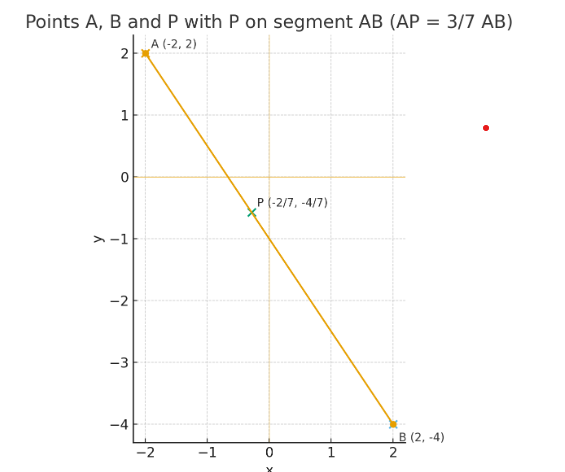
\includegraphics[width=0.6\columnwidth]{figs/plot1.png}
\end{center}

\end{document}